%\documentclass[handout,landscape]{beamer}
\documentclass[landscape]{beamer}
\hypersetup{pdfpagemode=FullScreen}
\mode<handout>
{
  \usepackage{pgf}
  \usepackage{pgfpages}

\pgfpagesdeclarelayout{6 on 1 boxed}
{
  \edef\pgfpageoptionheight{\the\paperheight} 
  \edef\pgfpageoptionwidth{\the\paperwidth}
  \edef\pgfpageoptionborder{0pt}
}
{
  \pgfpagesphysicalpageoptions
  {%
    logical pages=6,%
    physical height=\pgfpageoptionheight,%
    physical width=\pgfpageoptionwidth%
  }
  \pgfpageslogicalpageoptions{1}
  {%
    border code=\pgfsetlinewidth{2pt}\pgfstroke,%
    border shrink=\pgfpageoptionborder,%
    resized width=.5\pgfphysicalwidth,%
    resized height=.5\pgfphysicalheight,%
    center=\pgfpoint{.25\pgfphysicalwidth}{.833\pgfphysicalheight}%
  }%
  \pgfpageslogicalpageoptions{2}
  {%
    border code=\pgfsetlinewidth{2pt}\pgfstroke,%
    border shrink=\pgfpageoptionborder,%
    resized width=.5\pgfphysicalwidth,%
    resized height=.5\pgfphysicalheight,%
    center=\pgfpoint{.75\pgfphysicalwidth}{.833\pgfphysicalheight}%
  }%
  \pgfpageslogicalpageoptions{3}
  {%
    border code=\pgfsetlinewidth{2pt}\pgfstroke,%
    border shrink=\pgfpageoptionborder,%
    resized width=.5\pgfphysicalwidth,%
    resized height=.5\pgfphysicalheight,%
    center=\pgfpoint{.25\pgfphysicalwidth}{.5\pgfphysicalheight}%
  }%
  \pgfpageslogicalpageoptions{4}
  {%
    border code=\pgfsetlinewidth{2pt}\pgfstroke,%
    border shrink=\pgfpageoptionborder,%
    resized width=.5\pgfphysicalwidth,%
    resized height=.5\pgfphysicalheight,%
    center=\pgfpoint{.75\pgfphysicalwidth}{.5\pgfphysicalheight}%
  }%
  \pgfpageslogicalpageoptions{5}
  {%
    border code=\pgfsetlinewidth{2pt}\pgfstroke,%
    border shrink=\pgfpageoptionborder,%
    resized width=.5\pgfphysicalwidth,%
    resized height=.5\pgfphysicalheight,%
    center=\pgfpoint{.25\pgfphysicalwidth}{.167\pgfphysicalheight}%
  }%
  \pgfpageslogicalpageoptions{6}
  {%
    border code=\pgfsetlinewidth{2pt}\pgfstroke,%
    border shrink=\pgfpageoptionborder,%
    resized width=.5\pgfphysicalwidth,%
    resized height=.5\pgfphysicalheight,%
    center=\pgfpoint{.75\pgfphysicalwidth}{.167\pgfphysicalheight}%
  }%
}


  \pgfpagesuselayout{6 on 1 boxed}[letterpaper, border shrink=5mm]
  \nofiles
}

\usepackage{listings}
%\lstset{language=TeX}
\usepackage{multimedia}
\usepackage[normalem]{ulem}
\usepackage{amssymb}

%\usecolortheme[named=Purple]{structure} 
%\usetheme{Copenhagen}
\usetheme{Warsaw} 
\usecolortheme{seahorse}
\useoutertheme{infolines} 
%\usetheme[height=7mm]{Rochester} 
%\setbeamertemplate{items}[ball] 
\setbeamertemplate{blocks}[rounded][shadow=true] 
%\setbeamertemplate{navigation symbols}{} 
\author{Joe Fields}
\title{Introduction to Proof} 
%\subtitle{}
\date{Lecture 5}
\institute[SCSU]{ {\tt fieldsj1@southernct.edu} }

\newcommand{\versionNum}{$3.2$\ }

\newboolean{InTextBook}
\setboolean{InTextBook}{false}
\newboolean{InWorkBook}
\setboolean{InWorkBook}{false}
\newboolean{InHints}
\setboolean{InHints}{false}

%When this boolean is true (beginning in Section 5.1) we will use the convention
% that $0 \in \Naturals$.  If it is false we will continue to count $1$ as the smallest
%natural number (thus making Giuseppe Peano spin in his grave...)
 
\newboolean{ZeroInNaturals}

%This boolean is used to distinguish the version where we use $\sim$ rather than $\lnot$

\newboolean{LNotIsSim}

%The values of the last two booleans are set in ``switches.tex''

\setboolean{ZeroInNaturals}{true}
\setboolean{LNotIsSim}{false}


\let\savedlnot\lnot
\ifthenelse{\boolean{LNotIsSim}}{\renewcommand{\lnot}{\sim} }{}

%This command puts different amounts of space depending on whether we are
% in the text, the workbook or the hints & solutions manual. 
\newcommand{\twsvspace}[3]{%
 \ifthenelse{\boolean{InTextBook} }{\vspace{#1}}{%
  \ifthenelse{\boolean{InWorkBook} }{\vspace{#2}}{%
   \ifthenelse{\boolean{InHints} }{\vspace{#3}}{} %
   }%
  }%
 }


\newcommand{\wbvfill}{\ifthenelse{\boolean{InWorkBook}}{\vfill}{}}
\newcommand{\wbitemsep}{\ifthenelse{\boolean{InWorkBook} }{\rule[-24pt]{0pt}{60pt}}{}}
\newcommand{\textbookpagebreak}{\ifthenelse{\boolean{InTextBook}}{\newpage}{}}
\newcommand{\workbookpagebreak}{\ifthenelse{\boolean{InWorkBook}}{\newpage}{}}
\newcommand{\hintspagebreak}{\ifthenelse{\boolean{InHints}}{\newpage}{}}

\newcommand{\hint}[1]{\ifthenelse{\boolean{InHints}}{ {\par \hspace{12pt} \color[rgb]{0,0,1} #1 } }{}}
\newcommand{\inlinehint}[1]{\ifthenelse{\boolean{InHints}}{ { \color[rgb]{0,0,1} #1 } }{}}

\newlength{\cwidth}
\newcommand{\cents}{\settowidth{\cwidth}{c}%
\divide\cwidth by2
\advance\cwidth by-.1pt
c\kern-\cwidth
\vrule width .1pt depth.2ex height1.2ex
\kern\cwidth}

\newcommand{\sageprompt}{ {\tt sage$>$} }
\newcommand{\tab}{\rule{20pt}{0pt}}
\newcommand{\blnk}{\rule{1.5pt}{0pt}\rule{.4pt}{1.2pt}\rule{9pt}{.4pt}\rule{.4pt}{1.2pt}\rule{1.5pt}{0pt}}
\newcommand{\suchthat}{\; \rule[-3pt]{.5pt}{13pt} \;}
\newcommand{\divides}{\!\mid\!}
\newcommand{\tdiv}{\; \mbox{div} \;}
\newcommand{\restrict}[2]{#1 \,\rule[-4pt]{.25pt}{14pt}_{\,#2}}
\newcommand{\lcm}[2]{\mbox{lcm} (#1, #2)}
\renewcommand{\gcd}[2]{\mbox{gcd} (#1, #2)}
\newcommand{\Naturals}{{\mathbb N}}
\newcommand{\Integers}{{\mathbb Z}}
\newcommand{\Znoneg}{{\mathbb Z}^{\mbox{\tiny noneg}}}
\ifthenelse{\boolean{ZeroInNaturals}}{%
  \newcommand{\Zplus}{{\mathbb Z}^+} }{%
  \newcommand{\Zplus}{{\mathbb N}} }
\newcommand{\Enoneg}{{\mathbb E}^{\mbox{\tiny noneg}}}
\newcommand{\Qnoneg}{{\mathbb Q}^{\mbox{\tiny noneg}}}
\newcommand{\Rnoneg}{{\mathbb R}^{\mbox{\tiny noneg}}}
\newcommand{\Rationals}{{\mathbb Q}}
\newcommand{\Reals}{{\mathbb R}}
\newcommand{\Complexes}{{\mathbb C}}
%\newcommand{\F2}{{\mathbb F}_{2}}
\newcommand{\relQ}{\mbox{\textsf Q}}
\newcommand{\relR}{\mbox{\textsf R}}
\newcommand{\nrelR}{\mbox{\raisebox{1pt}{$\not$}\rule{1pt}{0pt}{\textsf R}}}
\newcommand{\relS}{\mbox{\textsf S}}
\newcommand{\relA}{\mbox{\textsf A}}
\newcommand{\Dom}[1]{\mbox{Dom}(#1)}
\newcommand{\Cod}[1]{\mbox{Cod}(#1)}
\newcommand{\Rng}[1]{\mbox{Rng}(#1)}

\DeclareMathOperator\caret{\raisebox{1ex}{$\scriptstyle\wedge$}}

\newtheorem*{defi}{Definition}
\newtheorem*{exer}{Exercise}
\newtheorem{thm}{Theorem}[section]
\newtheorem*{thm*}{Theorem}
\newtheorem{lem}[thm]{Lemma}
\newtheorem*{lem*}{Lemma}
\newtheorem{cor}{Corollary}
\newtheorem{conj}{Conjecture}

\renewenvironment{proof}%
{\begin{quote} \emph{Proof:} }%
{\rule{0pt}{0pt} \newline \rule{0pt}{15pt} \hfill Q.E.D. \end{quote}}


\newcommand{\vs}{\rule{0pt}{12pt}}

\AtBeginSection[]
{
 \begin{frame}{Table of Contents} 
  \tableofcontents[currentsection]
 \end{frame}
}

%%%% SAVE %%%%
%{ %magic to get a full screen image...
%\setbeamertemplate{navigation symbols}{}  % hide navigation buttons 
%\setbeamertemplate{background canvas}{\centerline{\includegraphics 
%	[height=\paperheight]{Cantor_4.jpeg}}}
%\begin{frame}[plain]
%\rule{0pt}{0pt}
%\end{frame} 
%} %end of magic


\begin{document}

\begin{frame}[plain]
  \titlepage
\end{frame}

\section{intro}

{ %magic to get a full screen image...
\setbeamertemplate{navigation symbols}{}  % hide navigation buttons 
\setbeamertemplate{background canvas}{\centerline{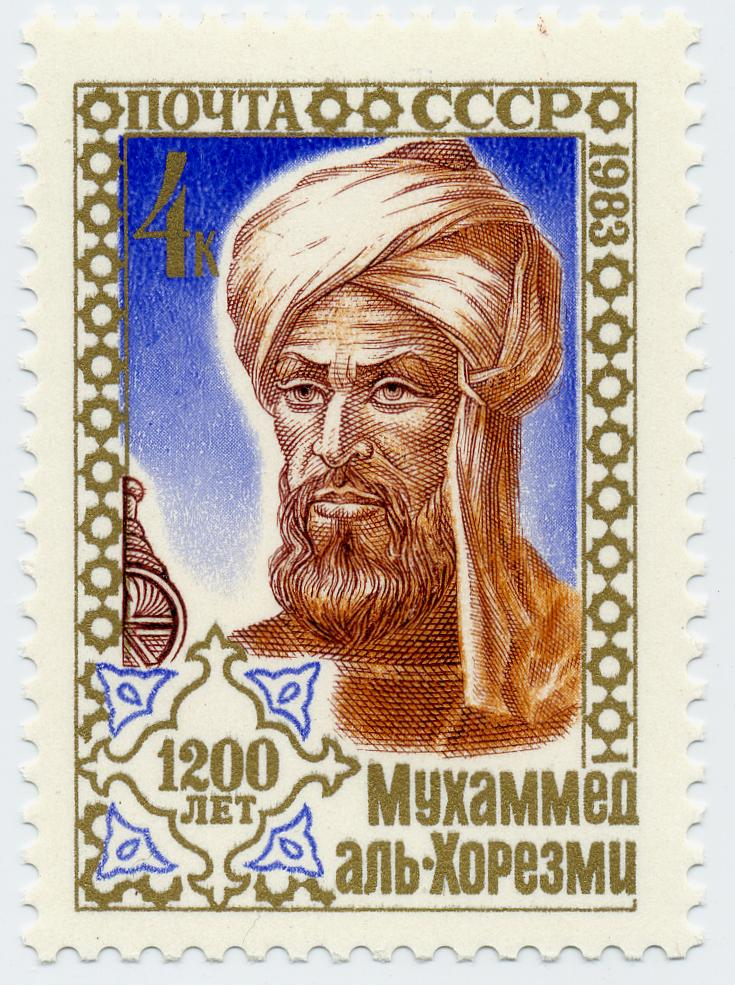
\includegraphics 
	[height=\paperheight]{khowar.jpg}}}
\begin{frame}[plain]
\rule{0pt}{0pt}
\end{frame} 
} %end of magic

\begin{frame}{a little history}
\begin{itemize}
\item Al-Khwarizmi\pause
\item Famous mathematician at the House of Wisdom in Baghdad. \pause
\item Coined the term (al-jabr) that eventually morphed into Algebra.\pause
\item Somehow his name got turned into Algoritmi when someone translated his work into Latin. \pause
\item Eventually, via more linguistic morphing we got Algorithm.
\end{itemize}
\end{frame}

\section{algorithms}

\begin{frame}{basics}
\begin{itemize}
\item An algorithm is simply a step-by-step procedure for accomplishing some task. \pause
\item A programmer goes to the grocery store\textellipsis \pause
\item Common elements:
\begin{itemize}
\item Assignments \pause
\item Tests and conditional execution \pause
\item Looping structures \pause
\item Returning a value
\end{itemize}
\end{itemize}
\end{frame}

\begin{frame}{forms suited to humans}
\begin{itemize}
\item Pseudocode \pause
\item Flowcharts \pause
\item XKCD \href{https://xkcd.com/627/}{https://xkcd.com/627/} and 
\href{https://xkcd.com/518/}{https://xkcd.com/518/}. \pause
\end{itemize}
\end{frame} 

\begin{frame}{tracing}
\begin{itemize}
\item Program "flow"\pause
\item Tracing a program\pause 
\item Trace tables\pause
\end{itemize}
\end{frame}

\section{the division algorithm}

\begin{frame}{The division algorithm}
\begin{center}
\begin{minipage}[b]{.5\textwidth}
\tt Algorithm: Division\\
Inputs: integers $n$ and $d$.\\
Local variables: $q$ and $r$.\\
\\
Let $q = 0$. \\
Let $r = n$. \\
Label 1.\\
If $r < d$ then\\
\rule{15pt}{0pt} Return $q$ and $r$.\\
End If\\
Let $q = q + 1$.\\
Let $r = r - d$.\\
Goto 1. \\
\end{minipage}
\end{center}
\end{frame}

\begin{frame}{A trace table for the division algorithm}
\begin{center}
Inputs: $n=33$ and $d=7$ \newline

\vspace{.1in}

\begin{tabular}{c|c|l} 
\rule[-6pt]{0pt}{24pt} \rule{12pt}{0pt} $q$ \rule{12pt}{0pt} & \rule{12pt}{0pt} $r$ \rule{12pt}{0pt} & Comments \\ \hline
\rule[-6pt]{0pt}{24pt}$0$ & $33$ & initialize the variables\\
\rule[-6pt]{0pt}{24pt}$1$ & $26$ & \\
\rule[-6pt]{0pt}{24pt}$2$ & $19$ & \\
\rule[-6pt]{0pt}{24pt}$3$ & $12$ & \\
\rule[-6pt]{0pt}{24pt}$4$ & $5$ & return $q=4$ and $r=5$ \\
\end{tabular}
\end{center}
\end{frame}

\section{gcd and lcm}

\begin{frame}{gcd}
\begin{itemize}
\item The greatest common divisor of two integers is (kinda like it says) the largest number that is a divisor of both of them. \pause
\item Example: Find the gcd of 105 and 231.\pause 
\item Divisors of 105: $\{1, 3, 5, 7, 15, 21, 35, 105 \}$.
\item Divisors of 231: $\{1, 3, 7, 11, 21, 33, 77, 231 \}$. \pause
\item The gcd is 21. \pause
\item This is even simpler if we look at the prime factorization of the numbers:

\[ 105 \; = \; 3 \cdot 5 \cdot 7 \quad \mbox{and} \quad 231 \; = \; 3 \cdot 7 \cdot 11 \]
\pause 
\item The gcd is just the product of the primes they have in common.
\end{itemize}
\end{frame}

\begin{frame}{lcm}
\begin{itemize}
\item Least Common Multiple\pause
\item Consider the sets of multiples of your numbers. (this is tougher since there are infinitely many!)\pause 
\item There have to be some in common between the two lists because the product of both numbers will certainly be on both lists.\pause
\item The smallest thing in common is the lcm.\pause
\item This number gets used often as a ``common denomenator.'' \pause

\[ \lcm{a}{b} = \frac{ab}{\gcd{a}{b}} \]
\end{itemize}
\end{frame}

\section{the Euclidean algorithm}

\begin{frame}{setup}
\begin{itemize}
\item Yes, that Euclid! \pause
\item If we had to factor numbers to find their gcd it would be more or less impossible to work with large numbers.\pause
\item As part of the public key cryptographic systems that enable internet commerce we need to be able to find the gcd of pairs of numbers having many hundreds of digits! \pause
\item Fortunately someone from Ancient Greece had already found a method. \pause
\item The key observation is that if $a > b$ and (using the division algorithm) we can write $a =qb+r$ then $\gcd{a}{b} = \gcd{b}{r}$. 
\end{itemize}
\end{frame}

\begin{frame}{the algorithm}
\begin{center}
\begin{minipage}[b]{.7\textwidth}
\tt Algorithm: Euclidean\\
Inputs: integers $a$ and $b$.\\
Local variables: $q$ and $r$.\\
\\
Label 1.\\
Let $(q,r)  = \mbox{Division}(a,b)$. \\
If $r = 0$ then\\
\rule{15pt}{0pt} Return $b$.\\
End If\\
Let $a = b$.\\
Let $b = r$.\\
Goto 1. \\
\end{minipage}
\end{center}
\end{frame}

\begin{frame}{A trace table for the Euclidean algorithm}
\begin{center}
Inputs: $a=341$ and $b=248$ \newline
\begin{tabular}{|c|c|c|c|l} 
\rule[-6pt]{0pt}{24pt} \rule{12pt}{0pt} $a$ \rule{12pt}{0pt} & \rule{12pt}{0pt} $b$ \rule{12pt}{0pt} & \rule{12pt}{0pt} $q$ \rule{12pt}{0pt} & \rule{12pt}{0pt} $r$ \rule{12pt}{0pt} & \\ \hline
\rule[-6pt]{0pt}{24pt}$341$ & $248$ & $0$ & $0$ & initialize the variables\\
\rule[-6pt]{0pt}{24pt}$341$ & $248$ & $1$ & $93$ & \\
\rule[-6pt]{0pt}{24pt}$248$ & $93$ & $2$ & $62$ & \\
\rule[-6pt]{0pt}{24pt}$93$ & $62$ & $1$ & $31$ & \\
\rule[-6pt]{0pt}{24pt}$62$ & $31$ & $2$ & $0$ & return\\
\end{tabular}
\end{center}
\end{frame}


\end{document}
